%!BIB program=biber

\documentclass{nkuthesis} % 普通毕业论文
%\documentclass[doublemajor]{nkuthesis} % 双学位毕业论文
%\documentclass[multiuline]{nkuthesis} % 

\usepackage{enumitem}
\setenumerate[1]{topsep=3pt,parsep=0pt}
\setitemize[1]{topsep=3pt,parsep=0pt}

\usepackage[backend=biber,style=gb7714-2015,gbnamefmt=lowercase]{biblatex}
\addbibresource{nkthesis.bib}
\DeclareBibliographyCategory{cited}
\AtEveryCitekey{\addtocategory{cited}{\thefield{entrykey}}}
\makeatletter
\DefineBibliographyStrings{english}{
	andothers   = {\protect\textit{et al}.},
	andothersincite={\protect\textit{et al}\adddot},
}
\makeatother
 % 此文件预引用了一些宏包,列出如下:enumitem,biblatex。读者无需重复引用。

% 使用文件预引用宏包的目的是方便对论文格式设定作调整,后续如有对论文模板的更新,方便替换文件。读者需要的宏包请在本文件导言区自行引用,如下
\usepackage{amsmath}
\usepackage{amssymb}

\usepackage{graphicx}
\graphicspath{{images/}}% 为了文件归类的便捷,请将论文需要插入的所有图片放到文件夹images里面

\usepackage{physics}

% 引用参考文献只需编写文件nkthesis.bib

\begin{document}
	% 设置基本信息
	% 注意:  逗号`,'是项目分隔符. 如果某一项的值出现逗号, 应放在花括号内, 如 {,}
	%
	\NKTsetup{%
		中文题目 = 论文标题,
		外文题目 = Title,
		学号     = xxxxxxx,
		姓名     = 学生,
		年级     = 大四,
		专业     = xx,
		系别     = 物理,
		学院     = xx学院,
		% 双修专业 = , %  如果是双学位,请去掉这两个注释
		% 双修院系 = ,
		指导教师 = xx教授,
		完成日期 =}
	
	% -*- coding: utf-8 -*-

\begin{abstractcn}
这是摘要。这是摘要。这是摘要。这是摘要。这是摘要。这是摘要。这是摘要。这是摘要。这是摘要。这是摘要。这是摘要。这是摘要。这是摘要。这是摘要。这是摘要。这是摘要。这是摘要。这是摘要。这是摘要。这是摘要。这是摘要。这是摘要。这是摘要。这是摘要。这是摘要。这是摘要。这是摘要。这是摘要。这是摘要。这是摘要。这是摘要。这是摘要。这是摘要。这是摘要。这是摘要。这是摘要。这是摘要。这是摘要。这是摘要。这是摘要。这是摘要。这是摘要。这是摘要。这是摘要。这是摘要。这是摘要。这是摘要。这是摘要。这是摘要。这是摘要。
\end{abstractcn}

\begin{keywordscn}
关、键、词、关键、词、关键词
\end{keywordscn}

\begin{abstract}
This is abstract.This is abstract.This is abstract.This is abstract.This is abstract.This is abstract.This is abstract.This is abstract.This is abstract.This is abstract.This is abstract.This is abstract.This is abstract.This is abstract.This is abstract.This is abstract.This is abstract.This is abstract.This is abstract.This is abstract.This is abstract.This is abstract.This is abstract.This is abstract.This is abstract.This is abstract.This is abstract.This is abstract.This is abstract.This is abstract.This is abstract.
\end{abstract}

\begin{keywords}
key,words,keywords
\end{keywords} 
	\tableofcontents
	% -*- coding: utf-8 -*-

\chapter{引言}
这是引言。这是引言。这是引言。这是引言。这是引言。这是引言。这是引言。这是引言。这是引言。这是引言。这是引言。这是引言。这是引言。这是引言。这是引言。这是引言。这是引言。这是引言。这是引言。这是引言。这是引言。这是引言。这是引言。这是引言。这是引言。这是引言。这是引言。这是引言。这是引言。这是引言。这是引言。这是引言。这是引言。这是\cite{test}引言。这是引言。这是引言。这是引言。这是引言。这是引言。这是引言。这是引言。这是引言。这是引言。这是引言。这是引言。这是引言。这是引言。这是引言。这是引言。这是引言。这是引言。这是引言。这是引言。这是引言。这是引言。


\chapter{模板简介}
本模板使用多文件结构,参与\LaTeX 编译的主要文件放在chapter子文件夹里,需要插入的图片文件等请放在images文件夹里。

本模板的标题,正文字体,页边距,目录,参考文献,行间距等主要论文格式已经设定完毕。
\section{封面}
封面样式已经设定完成,你只需要将封面对应信息填写在命令\verb|\NKTsetup|中即可。这一命令对应参数已经在main.tex文件中给出,请按需求填写。使用命令\verb|\NKTsetup|的同时本科生毕业论文的声明也将同时生成
\section{摘要与关键词}
摘要和关键词的相关信息请在abstract.tex中填写,摘要和关键词都需要中英文,中文摘要请在\verb|abstractcn|环境中填写,英文摘要请在\verb|abstract|环境中填写;中文关键词请在\verb|keywordscn|环境中填写,英文关键词请在\verb|keywords|环境中填写。
\section{目录}
目录由\verb|\tableofcontents|生成,这一命令已在main.tex中给出。在编译生成pdf的时候,为了生成正确的目录,可能需要编译2次。点击目录对应的标题可直接跳转至对应页面。
\section{正文}
正文内容请在mainbody.tex中填写。正文设有3个层级,章使用\verb|chapter|环境生成,节使用\verb|section|环境生成,小节使用\verb|subsection|环境生成。正文内容包括数学环境正常编辑即可。
\subsection{字体}
ctex宏集中提供了\verb|\songti|({\songti 宋体}),\verb|\heiti|({\heiti 黑体}),\verb|\fangsong|({\fangsong 仿宋}),\verb|\kaishu|({\kaishu 楷体})四种基本字体,如有需要请直接使用。另外本模板提供了\verb|\jiacu|({\jiacu 加粗})命令,在保持字体的基础上对其加粗。

如需要使用罗马数字,本模板提供了命令\verb|\Romannum|和\verb|\romannum|来分别生成大小写罗马数字。如\Romannum{2},\romannum{4}。
\subsection{字号}
字号请使用命令\verb|\zihao|来改变。如需要3号字,使用命令如{\zihao{3}这是三号字}。如需要对应的小号字,使用其相反数作为参数,如小3号字为{\zihao{-3}这是小三号字}。
\subsection{脚注}
脚注使用\verb|\footnote|生成,如\footnote{这是一个脚注}。
\subsection{图表}
本模板使用图表不采用浮动体形式,也即不使用环境\verb|figure|与\verb|table|,需要插入图片和表格时请使用\verb|center|环境。图片的标题使用\verb|\figurecaption|来生成,位于图片之下;表格的标题使用\verb|tablecaption|来生成,位于表格之上。如
\begin{center}
	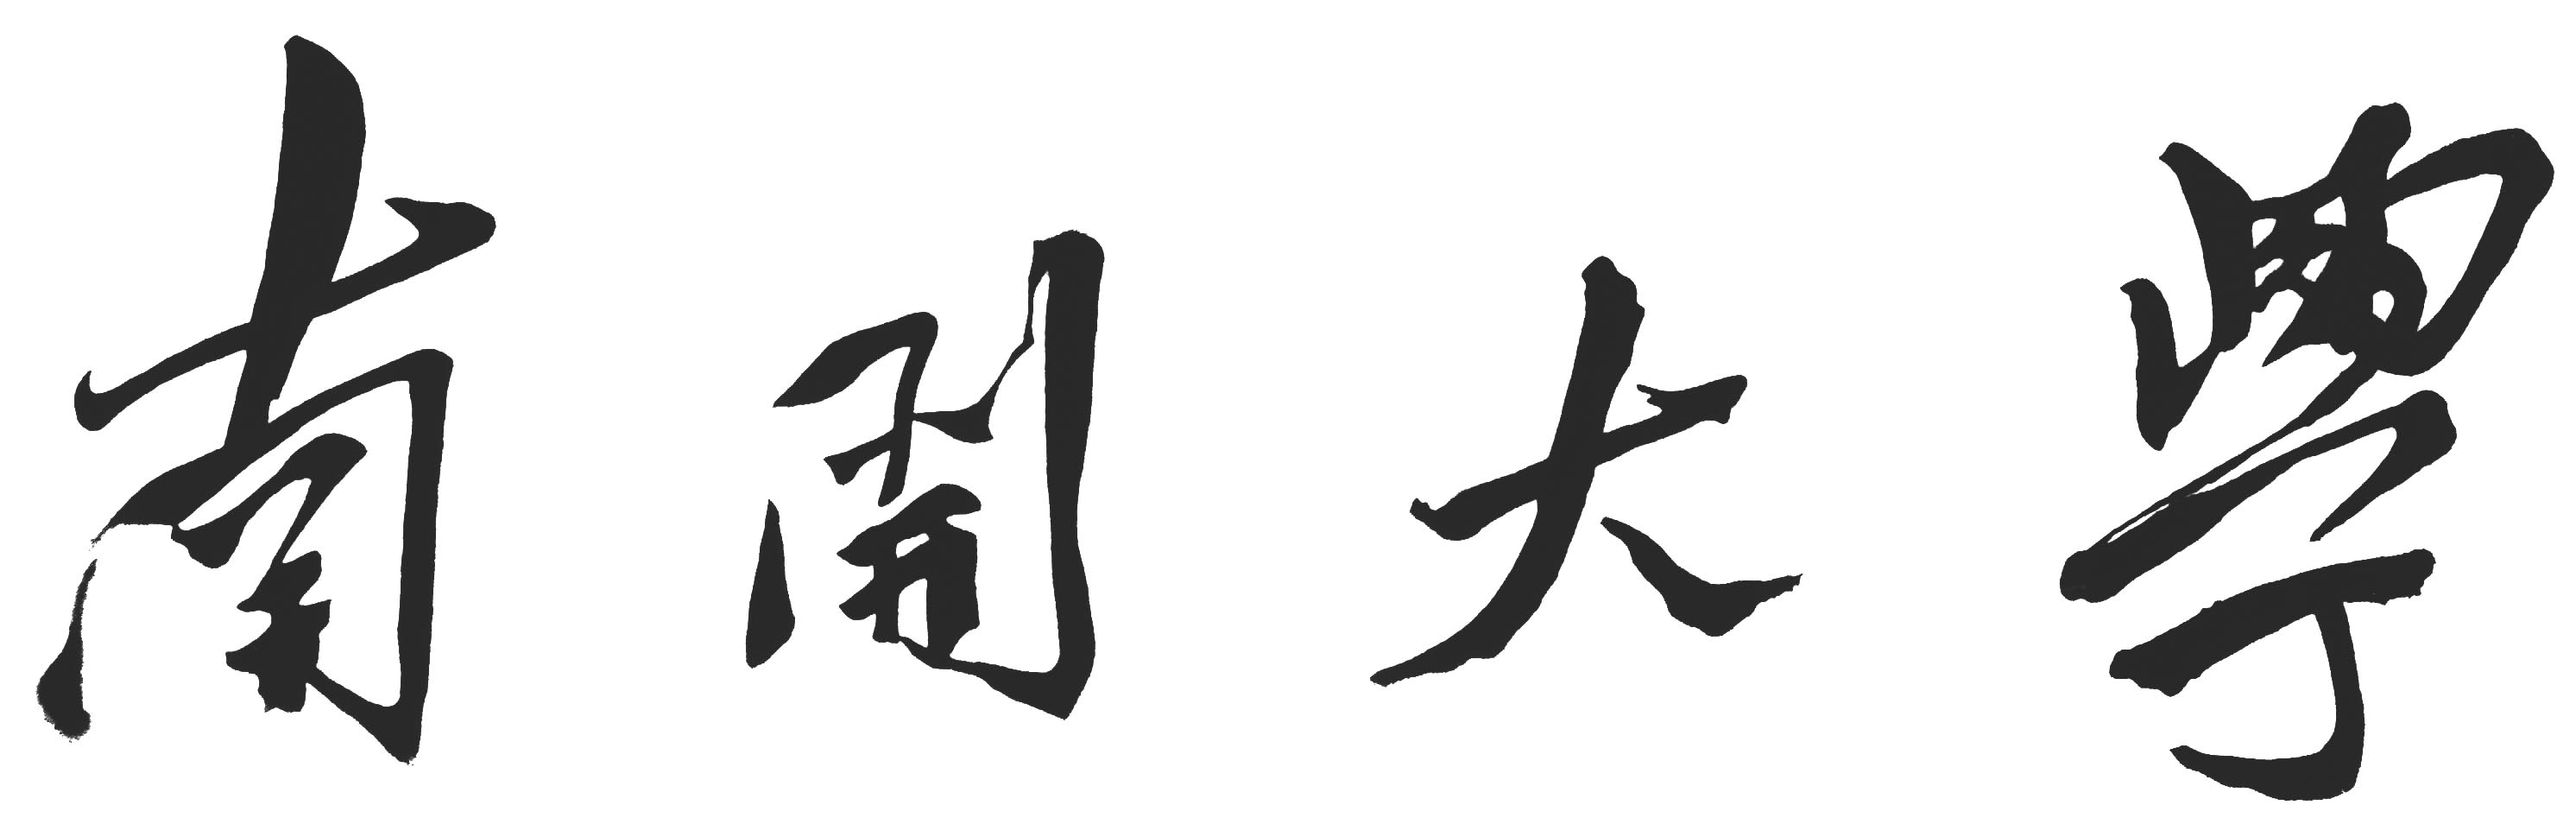
\includegraphics[height=2cm]{nankaidaxue.jpg}
	\figurecaption{这是标题}
\end{center}
如果想要同一行插入多张图片,共用一个标题,那么只需像下面这么写,可以控制中间需要空多宽
\begin{center}
	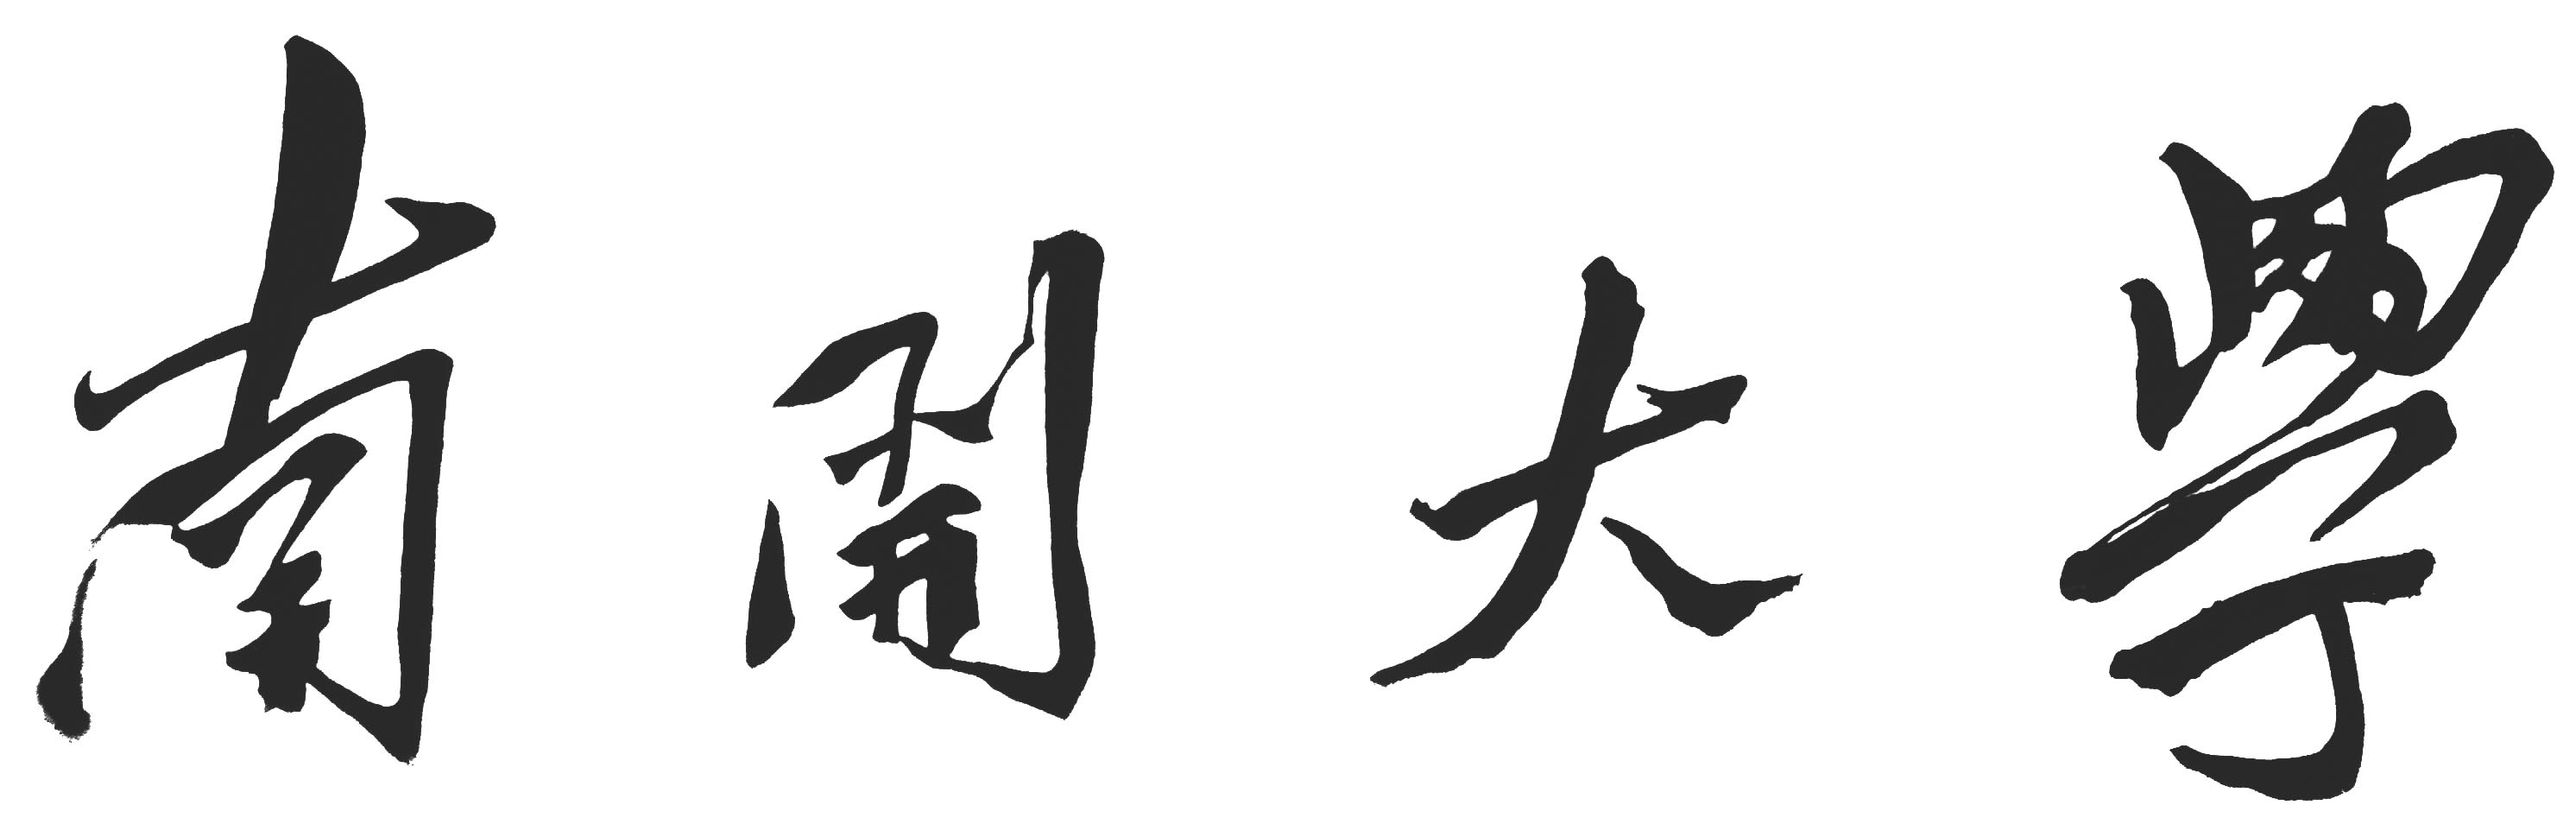
\includegraphics[height=2cm]{nankaidaxue.jpg}\hspace{0.8cm}
	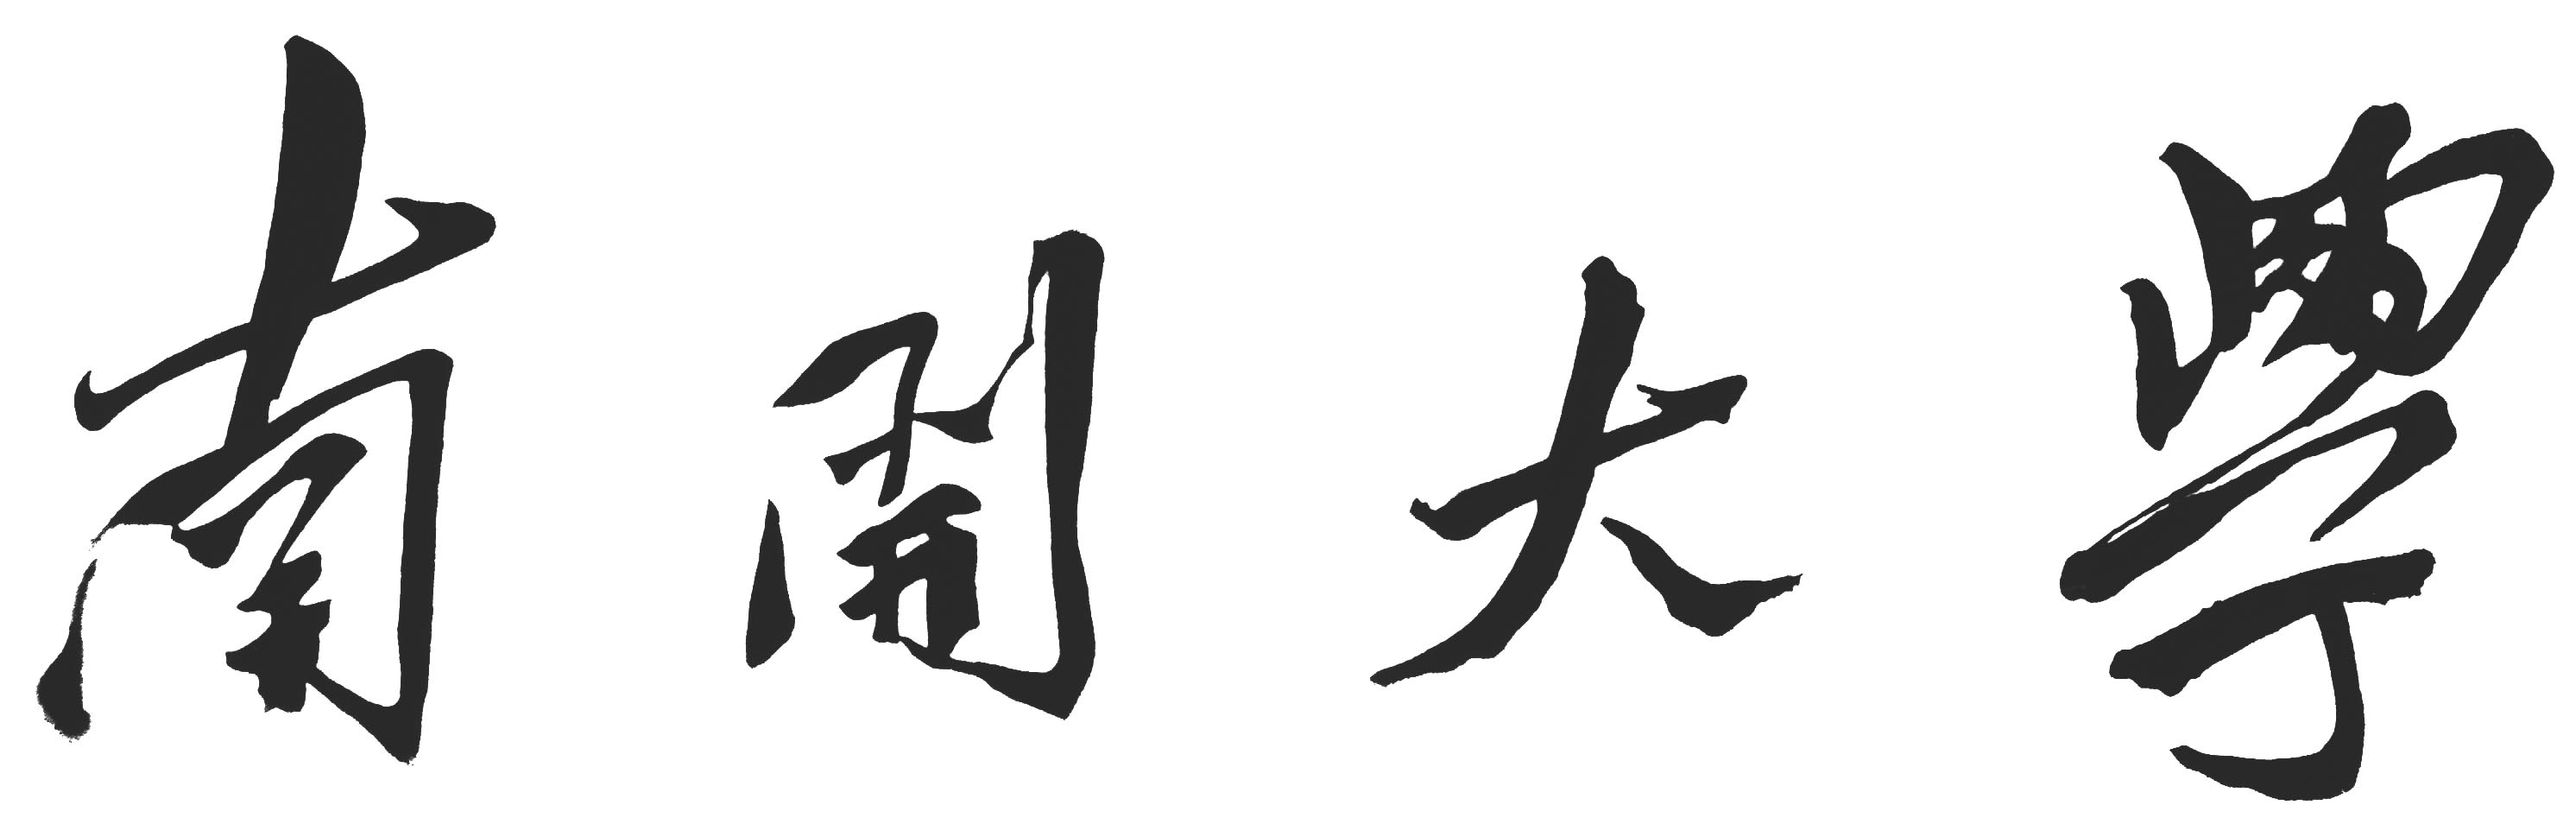
\includegraphics[height=2cm]{nankaidaxue.jpg}
	\figurecaption{这是标题}
\end{center}
特别注意论文格式要求中,表格一律采用三线表形式。如
\begin{center}
	\tablecaption{我是表格}
	\begin{tabular}{ccc}
		\hline
		条目一 & 条目二 & 条目三 \\ \hline
		内容一 &   1   &    2   \\
		内容二 &   2   &    2   \\
		内容三 &   3   &    3   \\
		内容四 &   4   &    4   \\ \hline
	\end{tabular}
\end{center}
\section{参考文献}
参考文献使用bib文件生成。如有需要的参考文献,你可以在相应的论文网站上导出bib格式,再将内容复制到文件nkthesis.bib中。引用文献一般使用\verb|\cite|命令,如\cite{zhaoliu},同时引用多个文件如\cite{zhaoliu,sunqian,chenjing,wuqiang}。同样,参考文献也需要多次编译才能正确生成,如果第一遍编译没法生成参考文献,请多再编译几次。参考文献对应的tex文件为references.tex,你不需要修改这一文件。

根据物理科学学院2018级毕业论文督察组的审核结果,光学组要求参考文献中,英文部分人名的首字母大写,其余小写。因此本模板在编写参考文献的时候,输入的时候大小写是什么,编译产生的大小写就是什么。比如你的输入为\verb|author={KoSeKi}|,那参考文献的作者部分输出就是KoSeKi。

注意:正文引用什么文献,后面的参考文献就按照正文引用的顺序自动生成;如果正文不引用某篇文献,那么后面参考文献将不显示这一篇。
\section{附录}
附录请在appendix.tex中填写。
\section{致谢}
致谢请在acknowledgements.tex中填写。
\section{个人简历}
个人简历请在resume.tex中填写。考虑到此命令不常用,默认注释掉。如有需求请在main.tex中取消对\verb|% -*- coding: utf-8 -*-

\chapter*{个人简历}
\maketoc{个人简历}

\noindent 姓名:xx\\
出生日期:2000年1月1日\\
\\
教育背景:\\
2018年9月-2022年7月\quad 南开大学\quad 物理科学学院\quad\quad\quad\quad 某某学\quad\quad 学士 \\
\\
本科期间发表的学术论文:\\
|命令的注释。
\begin{equation}
	2+6=8
\end{equation}
\begin{equation}
	1+1=2\hbar
\end{equation}
	% -*- coding: utf-8 -*-

{\bibstyle
\printbibliography[category = cited,title={参考文献}]
\maketoc{参考文献}
\clearpage}
	% -*- coding: utf-8 -*-

\chapter*{附\hspace{1em}录}
\maketoc{附录}
\appendix

这是你的附录内容。
\begin{equation}
	1+1=2
\end{equation}
	% -*- coding: utf-8 -*-

\chapter*{致\hspace{1em}谢}
\maketoc{致谢}

感谢使用本模板。
	%% -*- coding: utf-8 -*-

\chapter*{个人简历}
\maketoc{个人简历}

\noindent 姓名:xx\\
出生日期:2000年1月1日\\
\\
教育背景:\\
2018年9月-2022年7月\quad 南开大学\quad 物理科学学院\quad\quad\quad\quad 某某学\quad\quad 学士 \\
\\
本科期间发表的学术论文:\\

\end{document}